\chapter{SPEEDING UP THE FASTEST}
\label{sec:speedup}

As mentioned in Section \ref{sec:greedy}, \greedyAlgo\ has two main phases: PMF construction and reset word generation. The observations from Section \ref{sec:greedy-analysis} shows that in general, i.e., if the automata is not slowly synchronizing, the first phase dominates the execution time of the algorithm. However, to construct the reset word, the second phase does not use all the merging sequences obtained in the first phase. Therefore, the second phase can use a partial PMF. This observation establishes the base of our first optimization. 

In this section, we propose three algorithmic enhancements for \greedyAlgo\ algorithm. For the first improvement, the PMF construction is performed in a lazy manner, which is introduced in Section \ref{sec:lazy}. Section \ref{sec:lookahead} explains the second optimization on searching the merging sequences from a pair and is useful in the later stages. The last optimization, presented in Section \ref{sec:smart}, is minor and uses a basic idea to compute the intersection of the active pair set and a partial PMF.  

\section{Lazy PMF Construction}
\label{sec:lazy}

\greedyAlgo\ algorithm uses PMF to pick a shortest merging sequence among the set of current pairs ($C^{\langle2\rangle}$). However, Table \ref{table:levels} shows that the algorithm does not need to construct the whole PMF. It is redundant to compute the merging sequences whose length is longer than $h_{max}$. As the first improvement, we generated PMF in a lazy way and combined the two phases into a single one. Algorithm \ref{algo:greedy-lazy} searches a shortest merging sequence in PMF which is also a shortest merging sequence of a pair in $C^{\langle2\rangle}$. \greedyAlgo\ uses the partial PMF which initially contains only the merging sequences of the singletons. At each iteration, a new part of PMF is computed when it is needed. The algorithm checks all pairs in $C^{\langle2\rangle}$ to find a shortest merging sequence. If it does not find a merging sequence a PMF construction phase is initiated. This lazy process continues until a pair in $C^{\langle2\rangle}$ is found. After that it applies the merging sequence to all active pairs and continues with the next iteration. Note that the PMF construction is performed in a BFS-manner. Hence, the length of unidentified merging sequences cannot be shorter than the identified merging sequence in PMF.
 
\begin{algorithm}[ht]	
	\caption{\greedyAlgo\ algorithm with lazy PMF construction}
	\label{algo:greedy-lazy}
	
	\SetKwInOut{Input}{input}\SetKwInOut{Output}{output}
	\Input{An automaton ${\cal A}=(S,\Sigma,\delta)$}
	\Output{A synchronizing word $\Gamma$ for ${\cal A}$}
	\lForEach{singleton $\{ s,s \} \in S^{\langle 2 \rangle}$}{$\tau(\{s,s\}) = \varepsilon$}
	\lForEach{pair $\{ s_i,s_j \} \in S^{\langle 2 \rangle}$}{$\tau(\{ s_i,s_j \})${\em undefined}}
	$Q \longleftarrow \{ \{ s,s \}| s \in S \}$; \tcp{Q is a queue which will store unprocessed pair from frontier set and found pair from next frontier set.}
	$C = S$; \tcp{$C$ will keep track of the current set of states}
	$\Gamma = \varepsilon$; \tcp{$\Gamma$ is the synchronizing sequence to be constructed}
	\While{$|C| > 1$}	
	{
		\While{$\forall \{ s_i,s_j \} \in C^{\langle 2 \rangle}: \tau(\{ s_i,s_j \})$ is undefined}
		{
			$\{ s_i, s_j \} = $ dequeue the next item from $Q$\;
			\ForEach{$x \in \Sigma$}
			{
				\ForEach{$\{ s_k, s_\ell \} \in \delta^{-1}(\{ s_i, s_j \},x)$}
				{
					\If{$\tau(\{ s_k, s_\ell \})$ is undefined}
					{
						$\tau(\{ s_k, s_\ell \}) = x \; \tau(\{ s_i, s_j\})$\;
						enqueue $\{ s_k,s_\ell \}$ onto $Q$\;
					}
				}
			} 		
		}
		find a pair $\{ s_i, s_j \} \in C^{\langle 2 \rangle}$ 
		with a minimum $|\tau(\{ s_i,s_j \})|$ among all pairs 
		in $C^{\langle 2 \rangle}$\;
		$\Gamma = \Gamma \; \tau(\{ s_i, s_j \})$\;
		$C = \delta(C,\tau(\{ s_i,s_j\}))$;
	}
\end{algorithm}

In theory, Algorithm \ref{algo:greedy-lazy} has the same upper bound with Algorithm \ref{algo:greedy}. For lines 7-13, the time complexity depends on the number of edges which is $O(pn^2)$. The number of iterations does not have an impact on the complexity of lines 7-13. Also there is no lower bound for PMF construction. Picking a shortest merging sequence (lines 14-16) is performed in the same way as in Algorithm \ref{algo:greedy}. Therefore, the overall complexity is $O(n^4+ pn^2)$ and $\Omega(n)$. Thus the upper bound does not change but the lower bound decreases.

\section{Looking Ahead from the Current Pair}
\label{sec:lookahead}

As Section \ref{sec:lazy} describes, \greedyAlgo\ does not need a full PMF to find a shortest merging sequence at each iteration. Furthermore, Table \ref{table:levels} shows that the average length of a selected merging sequence is less than two. Hence, for most of the iterations, the algorithm picks a length-one merging sequence and it occasionally picks a merging sequence with a longer length, like $h_{max}$. Therefore, although such longer merging sequences are rare, Algorithm \ref{algo:greedy-lazy} still needs to construct PMF up to level $h_{max}$. In this section, a \textit{lookahead} technique is introduced to avoid constructing the deeper levels of PMF. The lookahead approach tries to find a shortest path from $C^{\langle 2 \rangle}$ to $Q$ via $\delta$~(instead of $\delta^{-1}$). Algorithm~\ref{algo:lookahead} and Figure~\ref{fig:lookahead} summarize the basic lookahead process.


\begin{algorithm}[ht]
	\caption{Looking ahead from $C^{\langle 2 \rangle}$}
	\label{algo:lookahead}
	
	\SetKwInOut{Input}{input}\SetKwInOut{Output}{output}
	\SetVlineSkip{0.1em}
	\setcounter{AlgoLine}{5}
	\nlset{$\mathbf{1..6}$} $\ldots$ \tcp{same as Algorithm~\ref{algo:greedy-lazy}} 
	\While{$|C| > 1$}	{
		\If{$\forall \{ s_i,s_j \} \in C^{\langle 2 \rangle}: \tau(\{ s_i,s_j \})$ is undefined} {
			\If{$|C| < $\sc{MaxStates}} {
				let $Q_L = C^{\langle 2 \rangle}$ and $Q_{L_2} = \emptyset$ be two queues\;	
				$q_{min} = \min_{\{ s_i, s_j \} \in Q} |\tau(\{ s_i, s_j \})|$; \\
				$cnt = 0$\;
			 	$\{ s_{k'},s_{\ell'}\}=$  {\em undefined}\;
			 	$\{ s_{k'_{root}},s_{\ell'_{root}}\}=$  {\em undefined}\;
				\lForEach{$\{ s_i, s_j \} \in S^{\langle 2 \rangle}$}{ $\sigma(\{ s_i, s_j \})  =$ {\em undefined}}
				\lForEach{$\{ s_i, s_j \} \in C^{\langle 2 \rangle}$}{$\sigma(\{ s_i, s_j \}) = \varepsilon$ and ${\{ s_{i_{root}},s_{j_{root}}\}}=\{s_i, s_j\}$}
				\While{$Q_L$ is not empty}{
					$\{ s_i, s_j \} = $ pop an item from $Q_L$\;\
				 	\For{$x \in \Sigma$} { 
						$\{ s_k, s_\ell \}$ = $\{ \delta(s_i,x), \delta(s_j,x)  \}$\;
						\If{$\sigma(\{ s_k, s_\ell \})$ is undefined}{
							push $\{ k, \ell \}$ to $Q_{L_2}$\;
							$\sigma(\{ s_k, s_\ell \}) = x \sigma(\{ s_i, s_j \})$\;
							${\{ s_{k_{root}}, s_{\ell_{root}} \}} = \{ s_{i_{root}}, s_{j_{root}} \}$\;
							$cnt++$;
						}
						\If{$\tau(\{ s_k, s_\ell \})$ is defined and $|\tau(\{ s_k, s_\ell \})| < |\tau(\{ s_{k'}, s_{\ell'} \})|$}{
							$\{ s_{k'}, s_{\ell'} \} = \{ s_k, s_\ell \}$	
						}
					}
					\If{$Q_L$ is empty and $cnt < ${\sc MaxPairs} and $\{ s_{k'},s_{\ell'}\}$ is undefined}{
						$Q_L = Q_{L_2}$ and $Q_{L_2} = \emptyset$;
					}
				}
				\If{${\{ s_{k'},s_{\ell'}\}}$ is defined}{
					use $\{ s_{k'_{root}},s_{\ell'_{root}}\}$ as $\{ s_i,s_j\}$ and $\sigma(\{ s_{k'}, s_{\ell'} \}) \tau(\{s_{k'},s_{\ell'} \})$ as $\tau(\{s_i,s_j \})$ for line 32-41
				}
			}
        	\While{$\forall \langle s_i,s_j \rangle \in C^{\langle 2 \rangle}: \tau(\{s_i,s_j \})$ is undefined} { 
        		\setcounter{AlgoLine}{37}
				\nlset{$\mathbf{33..38}$} $\ldots$ \tcp{same as lines 8-13 of Algo.~\ref{algo:greedy-lazy}}
			}
		}
		\setcounter{AlgoLine}{40}
		\nlset{$\mathbf{39..41}$} $\ldots$ \tcp{same as lines 14-16 of Algo.~\ref{algo:greedy-lazy}}
	}
\end{algorithm}

Let $\sigma_{\{  s_i, s_j \}}$ be the shortest path from $C^{\langle 2 \rangle}$ to $\{  s_i, s_j \}$ found by the lookahead process.  When $\tau(\{s_i,s_j \})$ is undefined for all $\{ s_i,s_j \} \in C^{\langle 2 \rangle}$, performing a lookahead fully and every time will be costly. To reduce the overhead, two constraints are defined; lookahead is allowed only when there are less than {\sc MaxStates}~(line 9) states in $C$ and it is allowed to traverse at most {\sc MaxPairs}~(line 16) pairs. We did not fine tune these parameters and use {\sc MaxStates} $= \log n$ and {\sc MaxPairs} $= n$. 

Although some bookkeeping can be applied, we never reuse the lookahead paths from the previous iteration~(see lines 15-16 in Algorithm~\ref{algo:lookahead}). We forget all the lookahead information once the process ends, because we want to continue exploring the forest level-by-level in a BFS fashion to keep the paths being shortest during the course of the overall heuristic. Furthermore, the current set of pairs changes in every iteration. The algorithm checks different pairs in each iteration. Therefore, the bookkeeping mechanism may not give a remarkable speed up. We decided not to implement the bookkeeping mechanism.

\begin{figure}[ht]
	\centering
	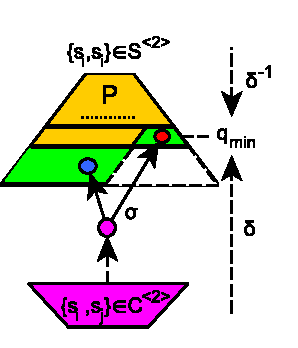
\includegraphics{figs/la.pdf}
	\caption{The figure summarizes the lookahead process: The BFS forest~(the top part of the figure) is being constructed via $\delta^{-1}$ in a lazy way. However, $P = \{ \{s_i, s_j \} | \tau(\{s_i, s_j \})~ \mbox{\em is defined} \}$ and $C^{\langle 2 \rangle}$ are disconnected. The process tries to find a shortest path from $C^{\langle 2 \rangle}$ to the queue $Q$~(the green colored BFS frontier). As an example, the $\sigma$ path passing through the blue $Q$ pair on the left is not the shortest one since there is a red $Q$ pair on the right which is reachable from the same purple lookahead pair. When the blue node is found, the current lookahead level (consisting of the nodes in $Q_L$) shall be completed to guarantee that the red node does (or does not) exist.}
	\label{fig:lookahead}
\end{figure}



\section{Reverse Intersection of the Active Pairs and PMF}
\label{sec:smart}

Algorithms \ref{algo:greedy-lazy} and \ref{algo:lookahead} frequently check if $\tau(\{ s_i,s_j \})$ is undefined or not for all the pairs in $C^{\langle 2 \rangle}$. Our baseline implementation traverses the pairs in $C^{\langle 2 \rangle}$ one by one and checks if they are in $P = \{ \{s_i, s_j \}\ |\ \tau(\{s_i, s_j \})~ \mbox{\em is defined} \}$. Although this is efficient when $|C^{\langle 2 \rangle}|$ is small, $|C^{\langle 2 \rangle}|$ is not small enough at the early stages of the algorithm. Hence, we reverse the search when $|C^{\langle 2 \rangle}| > |P|$ and traverse the pairs in $P$ and check if they are in $C^{\langle 2 \rangle}$.
